\documentclass[12pt]{article}
\usepackage[utf8]{inputenc}
\usepackage{polski}
\usepackage[a4paper, left=2.5cm, right=2.5cm, top=2.0cm, bottom=2.0cm]{geometry}
\usepackage{hyperref}
\usepackage{graphicx}

\title{GIT Cheat Sheet}
\author{mgr inż. Maciej Małecki\\ \small maciej.malecki@pwr.edu.pl}

\begin{document}
    \maketitle
    
    \section*{Instalacja narzędzi}
        Należy pobrać i~zainstalować wersję klienta GIT odpowiednią dla stosowanego systemu operacyjnego: \url{https://git-scm.com/downloads}.
        Klient ten zawiera narzędzia dostępne z linii poleceń i~jest wystarczający do pracy na zajęciach.

        Zalecane narzędzie graficzne nazywa się GitExtensions i~można je pobrać z~następującej strony: \url{https://github.com/gitextensions/gitextensions}.

    \section*{Konfiguracja dostępu SSH}
        Aby mieć dostęp do prywatnych repozytoriów GitHub, konieczna jest właściwa konfiguracja autentykacji. Zalecanym narzędziem jest OpenSSH (także w systemach Windows) oraz użycie pary kluczy RSA. OpenSSH dla systemu Windows jest dostarczane razem z~klientem GIT. Instrukcja generowania kluczy dostępna jest na GitHub\footnote{\url{https://help.github.com/articles/generating-a-new-ssh-key-and-adding-it-to-the-ssh-agent/\#generating-a-new-ssh-key}}.

        Wygenerowany klucz publiczny należy wgrać do ustawień swojego konta GitHub\footnote{\url{https://help.github.com/articles/adding-a-new-ssh-key-to-your-github-account/}}. W~przypadku, gdy posiadamy tylko jedno konto GitHub, wystarczające będzie skopiowanie klucza prywatnego do katalogu \texttt{users/<user name>/.ssh} pod nazwą \texttt{id\_rsa}.

    \subsection*{Dostęp SSH dla GitExtensions}
        W~przypadku klienta GitExtensions konieczne jest ustawienie OpenSSH jako metody autentykacji. Zmiany dokonujemy przy użyciu opcji menu \texttt{Settings/Git Extensions/SSH} (zobacz rys.~\ref{fig:gitext-ssh}). Wybór metody autentykacji możliwy jest także podczas instalacji narzędzia.
        \begin{figure}
            \centering
            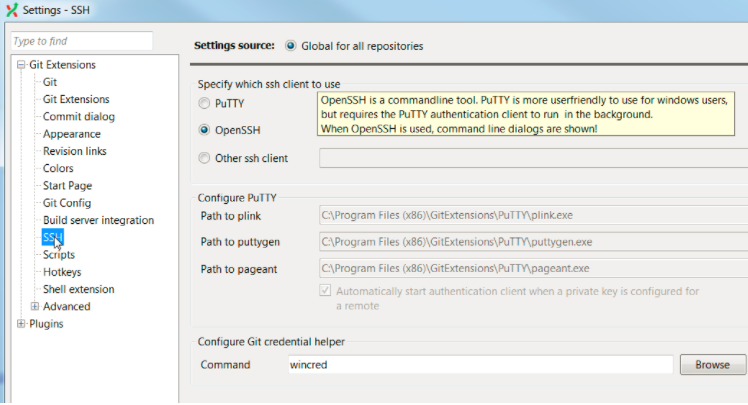
\includegraphics{gitextensions-ssh}
            \caption{Konfiguracja SSH w~kliencie GitExtensions.}
            \label{fig:gitext-ssh}
        \end{figure}

    \subsection*{Konfiguracja SSH dla wielu kont GitHub}\label{sec:ssh}
        W~przypadku, gdy posiadamy wiele kont w~portalu GitHub, możliwy jest wybór klucza prywatnego (a~więc i~użytkownika) dokonany dla każdego repozytorium oddzielnie. Przy założeniu, że dysponujemy oddzielnymi parami kluczy RSA dla każdego z~kont, konieczne jest utworzenie pliku config w katalogu \texttt{users/<user name>/.ssh} o~następującej zawartości:
        \begin{verbatim}
    Host priv
        HostName github.com
        User git
        IdentityFile ~/.ssh/id_rsa_priv
        IdentitiesOnly yes
    Host pwr
        HostName github.com
        User git
        IdentityFile ~/.ssh/id_rsa_pwr
        IdentitiesOnly yes
        \end{verbatim}
        \textbf{UWAGA}: dla każdego wpisu pole \texttt{User} zawsze musi mieć wartość \texttt{git}.

        Powyższy plik należy rozbudować o~kolejne wpisy w przypadku, gdy posiadamy więcej kont. Aby GIT (a~także GitExtensions) użył dedykowanego klucza prywatnego do dostępu do repozytorium, należy repozytorium sklonować używając nazwy \texttt{Host} z~pliku \texttt{config}, np.:
        \begin{verbatim}
    git clone pwr:pwr-piisw/oasp-seed
        \end{verbatim}
        sklonuje repozytorium \texttt{oasp-seed} wykorzystując użytkownika autentykowanego kluczem \texttt{id\_rsa\_pwr}. Natomiast:
        \begin{verbatim}
    git clone priv:pwr-piisw/oasp-seed
        \end{verbatim}
        dokona tego wykorzystując klucz \texttt{id\_rsa\_priv}.

    \section*{Praca z~GITem}
        Podstawowe komendy GITa przydatne w pracy nad projektem.
        \subsection*{Sklonowanie repozytorium}
        \begin{verbatim}
    git clone https://github.com/pwr-piisw/oaspseed
        \end{verbatim}
        lub
        \begin{verbatim}
    git clone pwr:pwr-piisw/oaspseed
        \end{verbatim}
        w~przypadku, gdy stosujemy wiele kluczy RSA; \texttt{pwr} jest wówczas wyróżnikiem klucza SSH.

        \subsection*{Konfiguracja repozytorium}
        Po sklonowaniu dobrze jest ustawić właściwie imię i~nazwisko użytkownika. Po wejściu do sklonowanego repozytorium możemy sprawdzić aktualną konfigurację przy pomocy komendy:
        \begin{verbatim}
    git config -l
        \end{verbatim}
        istotne są parametry \texttt{user.name} oraz \texttt{user.email}. Ich zmianę lokalną przeprowadzamy w~następujący sposób:
        \begin{verbatim}
    git config --add user.name "Maciej Małecki"
    git config --add user.email maciej.malecki@pwr.edu.pl
        \end{verbatim}
        Możliwa jest także zmiana globalna, działająca domyślnie dla wszystkich repozytoriów, najwygodniej w~tym celu użyć narzędzia w trybie edycji:
        \begin{verbatim}
    git config --global -e
        \end{verbatim}

        \subsection*{Pobieranie zdalnych zmian}
        Git jest narzędziem rozproszonym, lokalnie zawsze pracujemy na lokalnej kopii repozytorium. Aby zaktualizować jego zawartość, musimy użyć komendy \texttt{pull}, przy czym zawsze zalecane jest użycie trybu rebase:
        \begin{verbatim}
    git pull --rebase
        \end{verbatim}
        Tryb rebase wgra wszystkie zmiany zdalne ,,pod'' nasze zmiany, dzięki czemu zachowamy liniowość historii zmian (zwiększa to czytelność drzewa historii GITa). Operacja pull nie powiedzie się, jeśli mamy zmiany lokalne, które nie zostały dodane i~zatwierdzone do historii.

        \subsection*{Wprowadzanie zmian}
        Każde repozytorium GITa zawiera trzy obszary robocze:
        \begin{enumerate}
            \item Lokalny system plików
            \item \textit{Staging}
            \item Repozytorium
        \end{enumerate}
        Więcej szczegółów na \url{https://git-scm.com/book/en/v2/Getting-Started-Git-Basics}.

        Modyfikując pliki projektowe zawsze pracujemy na obszarze~1 (system plików). W~każdej chwili możemy sprawdzić status zmian przy użyciu:
        \begin{verbatim}
    git status
        \end{verbatim}
        Wybrane zmiany możemy dodać do obszaru~2 (\textit{staging}). Szczególnie wygodne jest tutaj narzędzie graficzne GitExtensions. W~przypadku linii poleceń stosujemy komendę add:
        \begin{verbatim}
    git add .
        \end{verbatim}
        aby dodać wszystkie zmiany z~systemu plików do \textit{staging} lub
        \begin{verbatim}
    git add doc/\*.txt
        \end{verbatim}
        aby dodać wszystkie pliki o~rozszerzeniu \texttt{txt} z~katalogu \texttt{doc}.
        Zatwierdzanie zmian (czyli dodanie ich do obszaru 3 - repozytorium) możliwe jest z~wykorzystaniem komendy \texttt{commit}:
        \begin{verbatim}
    git commit -m “Komentarz”
        \end{verbatim}
        Bardzo istotne jest stosowanie opisowych komentarzy do każdej zmiany.

        \subsection*{Przeglądanie zmian}
        Do przeglądania zmian w~repozytorium szczególnie przydatne jest narzędzie graficzne GitExtensions. Możliwe jest także użycie linii komend (więcej szczegółów: \url{https://git-scm.com/book/en/v2/Git-Basics-Viewing-the-Commit-History}). W~szczególności:
        \begin{verbatim}
    git log
        \end{verbatim}
        wyświetla listę ostatnich zmian w~repozytorium.
        \begin{verbatim}
    git log -p
        \end{verbatim}
        wyświetla listę zmian wraz z~wyszczególnieniem różnic w~plikach.
        \begin{verbatim}
    git log --graph --pretty=format:"%h - %an, %ar: %s"
        \end{verbatim}
        wyświetla listę zmian w~formie kompaktowej oraz z~wyszczególnieniem struktury drzewiastej.
        
        \subsection*{Aliasy}
        Wpisywanie długich poleceń (jak np.~\texttt{git log --graph --pretty=format:"\%h - \%an, \%ar: \%s"}) jest dość żmudne. Konfiguracja GIT'a umożliwia definiowanie skrótów (ang.~\textit{aliasów}). Na przykład:
        \begin{verbatim}
    git config --global alias.lp "log --graph 
                            --pretty=format:\"%h - %an, %ar: %s\""
        \end{verbatim}
        zdefiniuje skrót, który można następnie wywołać z~linii poleceń w~następujący sposób: \texttt{git lp}. W~przypadku systemów Unixowych, treść aliasa należy ująć w~apostrofy zamiast cudzysłowów.

        \subsection*{Anulowanie i~modyfikowanie zmian}
        Zmiany dokonane na lokalnym repozytorium mogą być w bezpieczny sposób anulowane lub zmodyfikowane. Jeśli zatwierdziliśmy zmianę, ale chcemy dodać coś jeszcze do tego commita, można to łatwo zrobić (dla ostatniego commita) przy użyciu:
        \begin{verbatim}
    git commit --amend
        \end{verbatim}
        W~podobny sposób można także zmienić komentarz do ostatniego commita:
        \begin{verbatim}
    git commit --amend -m "Nowy komentarz"
        \end{verbatim}
        Aby usunąć wszystkie niezatwierdzone zmiany (z~obszaru staging oraz z~lokalnego systemu plików) można użyć:
        \begin{verbatim}
    git reset --hard
        \end{verbatim}
        UWAGA: komenda ta trwale usuwa wszelkie lokalne i~niezatwierdzone zmiany bez prośby o~potwierdzenie! Więcej szczegółów: \url{https://git-scm.com/docs/git-reset}.

        \subsection*{Przenoszenie zmian na zdalne repozytorium}
        Wszelkie zatwierdzone zmiany muszą być scalone z repozytorium zdalnym na GitHub tak aby inni członkowie zespołu mieli do nich dostęp. Pierwszym etapem zawsze jest rebase, gdyż w każdej chwili mogą na zdalnym repozytorium pojawić się nowe zmiany. Rebase wykonujemy znaną nam już komendą pull:
        \begin{verbatim}
    git pull --rebase
        \end{verbatim}
        Podczas tej operacji możliwy jest konflikt (czyli sytuacja, w~której dwie osoby dokonały w~tym samym czasie modyfikacji tego samego fragmentu kodu). Do rozwiązywania konfliktów najwygodniej użyć narzędzia GitExtensions z~zainstalowanym pluginem KDiff3 (zobacz rysunek~\ref{fig:gitext-kdiff3}).
        \begin{figure}
            \centering
            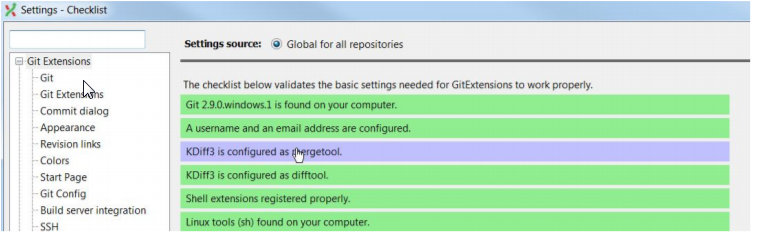
\includegraphics{gitextensions-kdiff3}
            \caption{Konfiguracja narzędzia do scalania w~kliencie GitExtensions.}
            \label{fig:gitext-kdiff3}
        \end{figure}
        Rozwiązywanie konfliktów w większości przypadków następuje automatycznie. Ingerencja potrzebna jest tylko tam, gdy narzędzie nie potrafi samo zdecydować jak powinien wyglądać kod po scaleniu (np modyfikacja dotyczyła tej samej linijki kodu)\footnote{Polecam lekturę: \url{https://git-scm.com/book/en/v2/Git-Branching-Basic-Branching-and-Merging}.}. Po rozwiązaniu wszelkich konfliktów zmiany należy jak najszybciej przenieść na zdalne repozytorium:
        \begin{verbatim}
    git push
        \end{verbatim}
        Oczywiście, w~sytuacji, gdy w~czasie rozwiązywania konfliktów na repozytorium zdalnym pojawiły się nowe zmiany, \texttt{git push} się nie powiedzie i~proces rebase oraz rozwiązywania konfliktów musi być powtórzony.

        \subsection*{Praca z~gałęziami}
        Gałęzie (ang. \textit{branches}) tworzą rozwidlenie drzewa wersji i~pozwalają na równoległą pracę nad kodem przez wiele osób. Gałęzie używane są także w~procesie wersjonowania i~wydawania kodu aplikacji. Utworzenie gałęzi umożliwia komenda:
        \begin{verbatim}
    git branch <branch name>
        \end{verbatim}
        gdzie \texttt{branch name} określa nazwę nowotworzonej gałęzi. Rozwidlenie zostanie utworzone w~miejscu wskazywanym przez wskaźnik \texttt{HEAD}. Po utworzeniu możliwe jest przejście na utworzoną gałąź przy pomocy komendy: \texttt{git checkout <branch name>}. Odtąd zmiany wprowadzane będą bezpośrednio na wybranej gałęzi.

        Istnieją zasadniczo dwie metody integracji dwóch gałęzi. W~przypadku gdy chcemy przenieść zmiany z~jednej gałęzi do drugiej (z~reguły druga gałąź jest gałęzią, z~której nastąpiło rozwidlenie) wykorzystujemy operację \textit{merge}: \texttt{git merge <branch>} (zobacz rysunek~\ref{fig:git-merge}).

        \begin{figure}[ht]
            \centering
            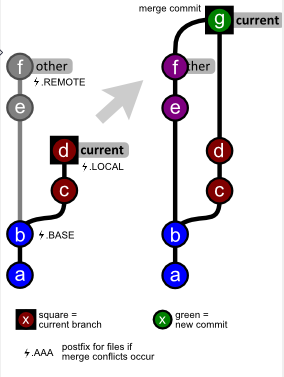
\includegraphics{git-merge}
            \caption{Integracja zmian poprzez \textit{merge}.}
            \label{fig:git-merge}
        \end{figure}

        W~sytuacji w~której chcemy wprowadzić do gałęzi potomnej zmiany z~gałęzi bazowej dokonane po momencie rozwidlenia, używamy operacji \textit{rebase}: \texttt{git rebase <branch>} (zobacz rysunek~\ref{fig:git-rebase}). Operacja \textit{rebase} powoduje nadpisanie historii i~należy używać jej z~rozwagą podczas pracy na gałęziach współdzielonych (wypushowywanie takiej gałęzi wymaga użycia opcji \texttt{--force}).

        \begin{figure}[ht]
            \centering
            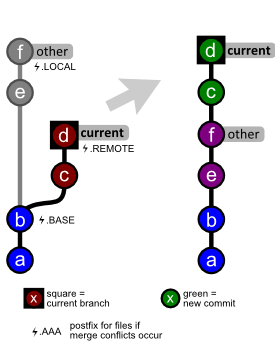
\includegraphics{git-rebase}
            \caption{Integracja zmian poprzez \textit{rebase}.}
            \label{fig:git-rebase}
        \end{figure}

        \subsection*{Tagowanie}
        W~trakcie prac laboratoryjnych oraz oddawania poszczególnych etapów prosimy o~tagowanie zmian, które podlegają ocenie. Tagi wymagają oddzielnego pushowania do zdalnego repozytorium. Tag jest etykietą posiadającą nazwę i~jest przypisany do konkretnego commita w historii.

        Poniższa komenda:
        \begin{verbatim}
    git tag lab03
        \end{verbatim}
        utworzy tag o nazwie \texttt{lab03} na najświeższym commicie. Alternatywnie możliwe jest tagowanie starszych commitów z~przy pomocy następującej komendy:
        \begin{verbatim}
    git tag lab03 <commit sha>
        \end{verbatim}
        gdzie "commit sha" jest skrótem, który możemy odczytać np. przy użyciu komendy (jest to zawartość pierwszej kolumny - 7-mio cyfrowa liczba heksadecymalna):
        \begin{verbatim}
    git log --pretty=format:"%h - %an, %ar: %s"
        \end{verbatim}
        Utworzony tag należy następnie wypushować do zdalnego repozytorium (nie dzieje się to automatycznie, nie robi tego też komenda git push bez dodatkowych parametrów):
        \begin{verbatim}
    git push origin lab03
        \end{verbatim}

\end{document}